%
% $Id: slides.tex 4228 2010-12-02 17:55:12Z pcoca $
%
%
% Compilar a .pdf con LaTeX (pdflatex)
% Es necesario instalar Beamer (paquete latex-beamer en Debian)
%

%
% Gráficos:
% Los gráficos pueden suministrarse en PNG, JPG, TIF, PDF, MPS
% Los EPS deben convertirse a PDF (usar epstopdf)
%

\documentclass{beamer}
\usetheme{Warsaw}
\usebackgroundtemplate{
\includegraphics[width=\paperwidth]{format/libresoft-bg.png}}
\usepackage[spanish]{babel}
\usepackage[utf8]{inputenc}
\usepackage{graphics}
\usepackage{amssymb} % Simbolos matematicos
\usepackage{url}

%\definecolor{libresoftgreen}{RGB}{162,190,43}
%\definecolor{libresoftblue}{RGB}{0,98,143}

%\setbeamercolor{titlelike}{bg=libresoftgreen}

%% Metadatos del PDF.
\hypersetup{
  pdftitle={FLOSS Testing and Quality Assurance},
  pdfauthor={F. Ortega, D. Izquierdo, P. Coca, P. García}
  pdfcreator={GSyC/Libresoft},
  pdfproducer=PDFLaTeX,
  pdfsubject={nn},
}
%%


\AtBeginSection[]
{
  \begin{frame}<presentation>
    \frametitle{Index}
    \tableofcontents[current]
  \end{frame}
}


\begin{document}

\title{FLOSS Testing and Quality Assurance}
\subtitle{Mozilla Thunderbird}
\institute{\\pcoca@libresoft.es\\
GSyC/Libresoft}
\author{Felipe Ortega, Daniel Izquierdo, Pedro Coca, Pedro García}
\date{\today}

\frame{
\maketitle
\begin{center}

\includegraphics[width=6cm]{format/gsyc-urjc}
\end{center}
}


% Si el titulo o el autor se quieren acortar para los pies de página
% se pueden redefinir aquí:
%\title{Titulo corto}
%\author{Autores abreviado}


%% LICENCIA DE REDISTRIBUCION DE LAS TRANSPAS
\frame{
~
\vspace{4cm}

\begin{flushright}
{\tiny
(cc) 2010 Felipe Ortega, Daniel Izquierdo, Pedro Coca, Pedro García. \\
Some rights reserved. This document is distributed under the Creative \\
            Commons Attribution-ShareAlike 3.0 licence, available in \\
            http://creativecommons.org/licenses/by-sa/3.0/

%  Este documento (o uno muy similar) está disponible en \\
%  \url{http://gsyc.escet.urjc.es/~jjamor/}
}
\end{flushright}
}
%%

%%%%%%
%Transpas separadas por \begin{frame}
%%%%%%%%%%%%%%%%%%%%%%%%\end{frame}

\section{Introduction}

\begin{frame}
\frametitle{What is QA}
\begin{itemize}
\item Trackin and monitoring the software engineering processes
    \begin{itemize}
       \item software design 
       \item source code control 
       \item change management 
       \item ...
       \item configuration management 
       \item testing 
       \item release management
    \end{itemize}
\item Goal: Ensure "Quality"
\item As we have seen before, some standards, methodologies and paradigms aim partially or totally this goal
\end{itemize}
\end{frame}

%%%%%%%%%%%%%%%%%%%%%%%%%%%%%%%%%%%%%%%%%%%%%%%%%%%%%%%%%%%%%%

\section{Introduction to Mozilla}

%%%%%%%%%%%%%%%%%%%%%%%%%%%%%%%%%%%%%%%%%%%%%%%%%%%%%%%%%%%%%%

\begin{frame}
\frametitle{What is Mozilla?}
 \begin{itemize}
 \item The Mozilla Foundation is a non-profit organization that exists to support and provide leadership for the Open Source Mozilla project
 \item The Mozilla Foundation is formed by two subsidiaries:
     \begin{itemize}
     \item Mozilla Corporation, founded in 2005. Develops the Mozilla Firefox web browser
     \item Mozilla Messaging, founded in 2008. Develops the Mozilla Thunderbird email client
     \end{itemize}

 \end{itemize}
\end{frame}


\section{Mozilla QA}
%%%%%%%%%%%%%%%%%%%%%%%%%%%%%%%%%%%%%%%%%%%%%%%%%%%%%%%%%%%%%%

\begin{frame}
\frametitle{Mozilla QA structure}
\begin{center}
 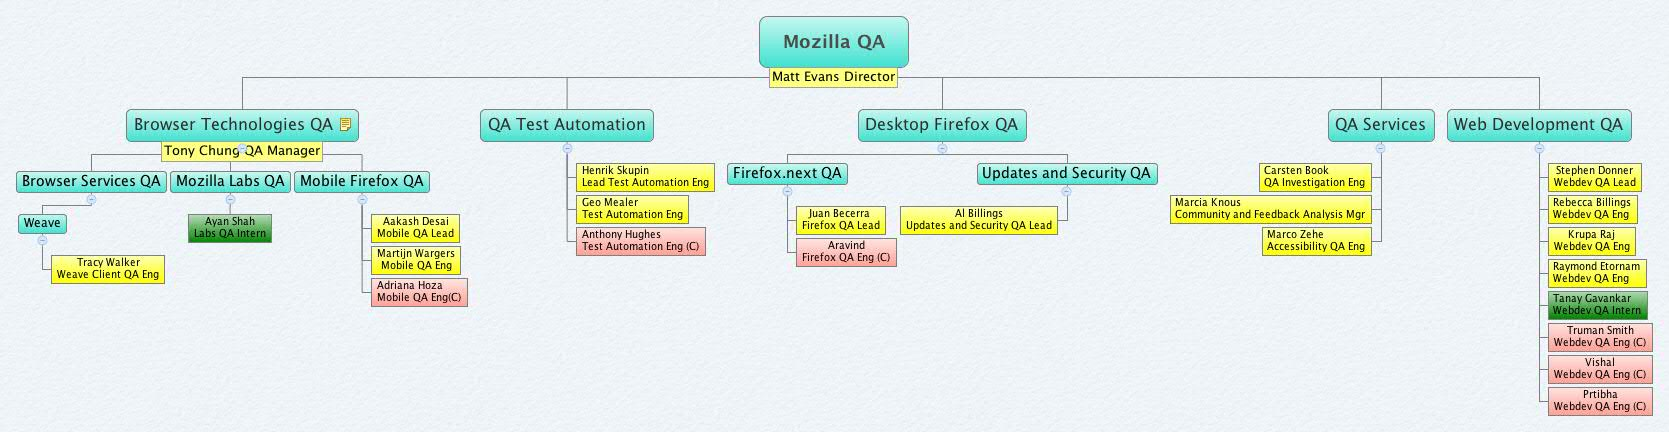
\includegraphics[height=5cm,width=11.5cm]{figs/MozillaQAOrgPic.jpg}
\begin{figure}
\end{figure}
\end{center}
\end{frame}

%%%%%%%%%%%%%%%%%%%%%%%%%%%%%%%%%%%%%%%%%%%%%%%%%%%%%%%%%%%%%%

%%%%%%%%%%%%%%%%%%%%%%%%%%%%%%%%%%%%%%%%%%%%%%%%%%%%%%%%%%%%%%

\section{Introduction to Thunderbird}

%%%%%%%%%%%%%%%%%%%%%%%%%%%%%%%%%%%%%%%%%%%%%%%%%%%%%%%%%%%%%%

\begin{frame}
\frametitle{What is Thunderbird?}
 \begin{itemize}
 \item Thunderbird is a Free/Libre/Open Source Cross-Platform email and news client
 \item Runs on Windows, Linux, MacOS X, OS/2, OpenSolaris, etc
 \end{itemize}
\end{frame}


%%%%%%%%%%%%%%%%%%%%%%%%%%%%%%%%%%%%%%%%%%%%%%%%%%%%%%%%%%%%%%

\begin{frame}
 \frametitle{Thunderbird Features}
 \begin{itemize}
 \item Message management
 \item Tabs
 \item Mail Account Setup Wizard
 \item One-click Address Book
 \item Attachment Reminder
 \item Activity Manager
 \item Offline operation
 \item Message Search
 \item Add-ons (Calendar, etc)
 \end{itemize}
\end{frame}

%%%%%%%%%%%%%%%%%%%%%%%%%%%%%%%%%%%%%%%%%%%%%%%%%%%%%%%%%%%%%%

\begin{frame}
 \frametitle{Thunderbird Licenses}
 \begin{itemize}
 \item Mozilla is released under several FLOSS Licences
 \item Triple licensing:
    \begin{itemize}
     \item LGPL
     \item GPLv2
     \item Mozilla Public License 1.1
    \end{itemize}

 \end{itemize}
\end{frame}

%%%%%%%%%%%%%%%%%%%%%%%%%%%%%%%%%%%%%%%%%%%%%%%%%%%%%%%%%%%%%%

\begin{frame}
 \frametitle{Versions}
 \begin{itemize}
 \item Initial release
    \begin{itemize}
     \item 0.1. July 2003
    \end{itemize}

 \item Current stable release (December 2010)
    \begin{itemize}
     \item 3.1.6. October 2010
    \end{itemize}

 \item Latest alpha release (December 2010)
    \begin{itemize}
     \item 3.3.a1 November 2010
    \end{itemize}

 \end{itemize}
\end{frame}

%%%%%%%%%%%%%%%%%%%%%%%%%%%%%%%%%%%%%%%%%%%%%%%%%%%%%%%%%%%%%%

\begin{frame}
 \frametitle{Versions}
 \begin{itemize}
 \item First and Second digit means major releases
 \item Third digit means security and stability releases
 \item Initial release
    \begin{itemize}
     \item 0.1. July 2003
    \end{itemize}

 \item First mayor release 0.1
    \begin{itemize}
     \item 1.0. December 2004
    \end{itemize}

 \item Second mayor release 0.1
    \begin{itemize}
     \item 2.0. April 2007
    \end{itemize}

 \item Third mayor release 0.1
    \begin{itemize}
     \item 3.0. December 2009
    \end{itemize}

 \end{itemize}
\end{frame}

%%%%%%%%%%%%%%%%%%%%%%%%%%%%%%%%%%%%%%%%%%%%%%%%%%%%%%%%%%%%%%

\begin{frame}
\frametitle{Software Metrics}
 \begin{itemize}
 \item About 1.000.000 lines of code
 \item Programming Languages
    \begin{itemize}
     \item C++
     \item Javascript
     \item XML
     \item Java
     \item C
     \item Others
    \end{itemize}
 \item Almost 600 contributors
 \item 6 Million daily users
 \end{itemize}
\end{frame}

%%%%%%%%%%%%%%%%%%%%%%%%%%%%%%%%%%%%%%%%%%%%%%%%%%%%%%%%%%%%%%

\begin{frame}
 \frametitle{Mozilla QA}
 \begin{itemize}
 \item QA is the method to evaluate and monitor several aspect of a software project
 \item Mozilla QA uses tools such as:
    \begin{itemize}
     \item Bugzilla
     \item Crash reporter
     \item Manual software testing
     \item Automated software testing 
    \end{itemize}
 \end{itemize}
\end{frame}

%%%%%%%%%%%%%%%%%%%%%%%%%%%%%%%%%%%%%%%%%%%%%%%%%%%%%%%%%%%%%%
\section{Testing tools}

\begin{frame}
 \frametitle{Mozilla QA Tools: Bugzilla}
 \begin{itemize}
 \item Web based bug tracker originally developed to be used by the Mozilla project
 \item Released under the MPL
 \item Released as FLOSS in 1998 by Netscape
 \item It is used by many important FLOSS projects/companies
    \begin{itemize}
    \item GhostScript
    \item Novell
    \item Songbird
    \item Gnome
    \item Apache
    \item ...
    \end{itemize}
 \end{itemize}
\end{frame}

%%%%%%%%%%%%%%%%%%%%%%%%%%%%%%%%%%%%%%%%%%%%%%%%%%%%%%%%%%%%%%

\begin{frame}
\frametitle{Mozilla Usage}
\begin{center}
 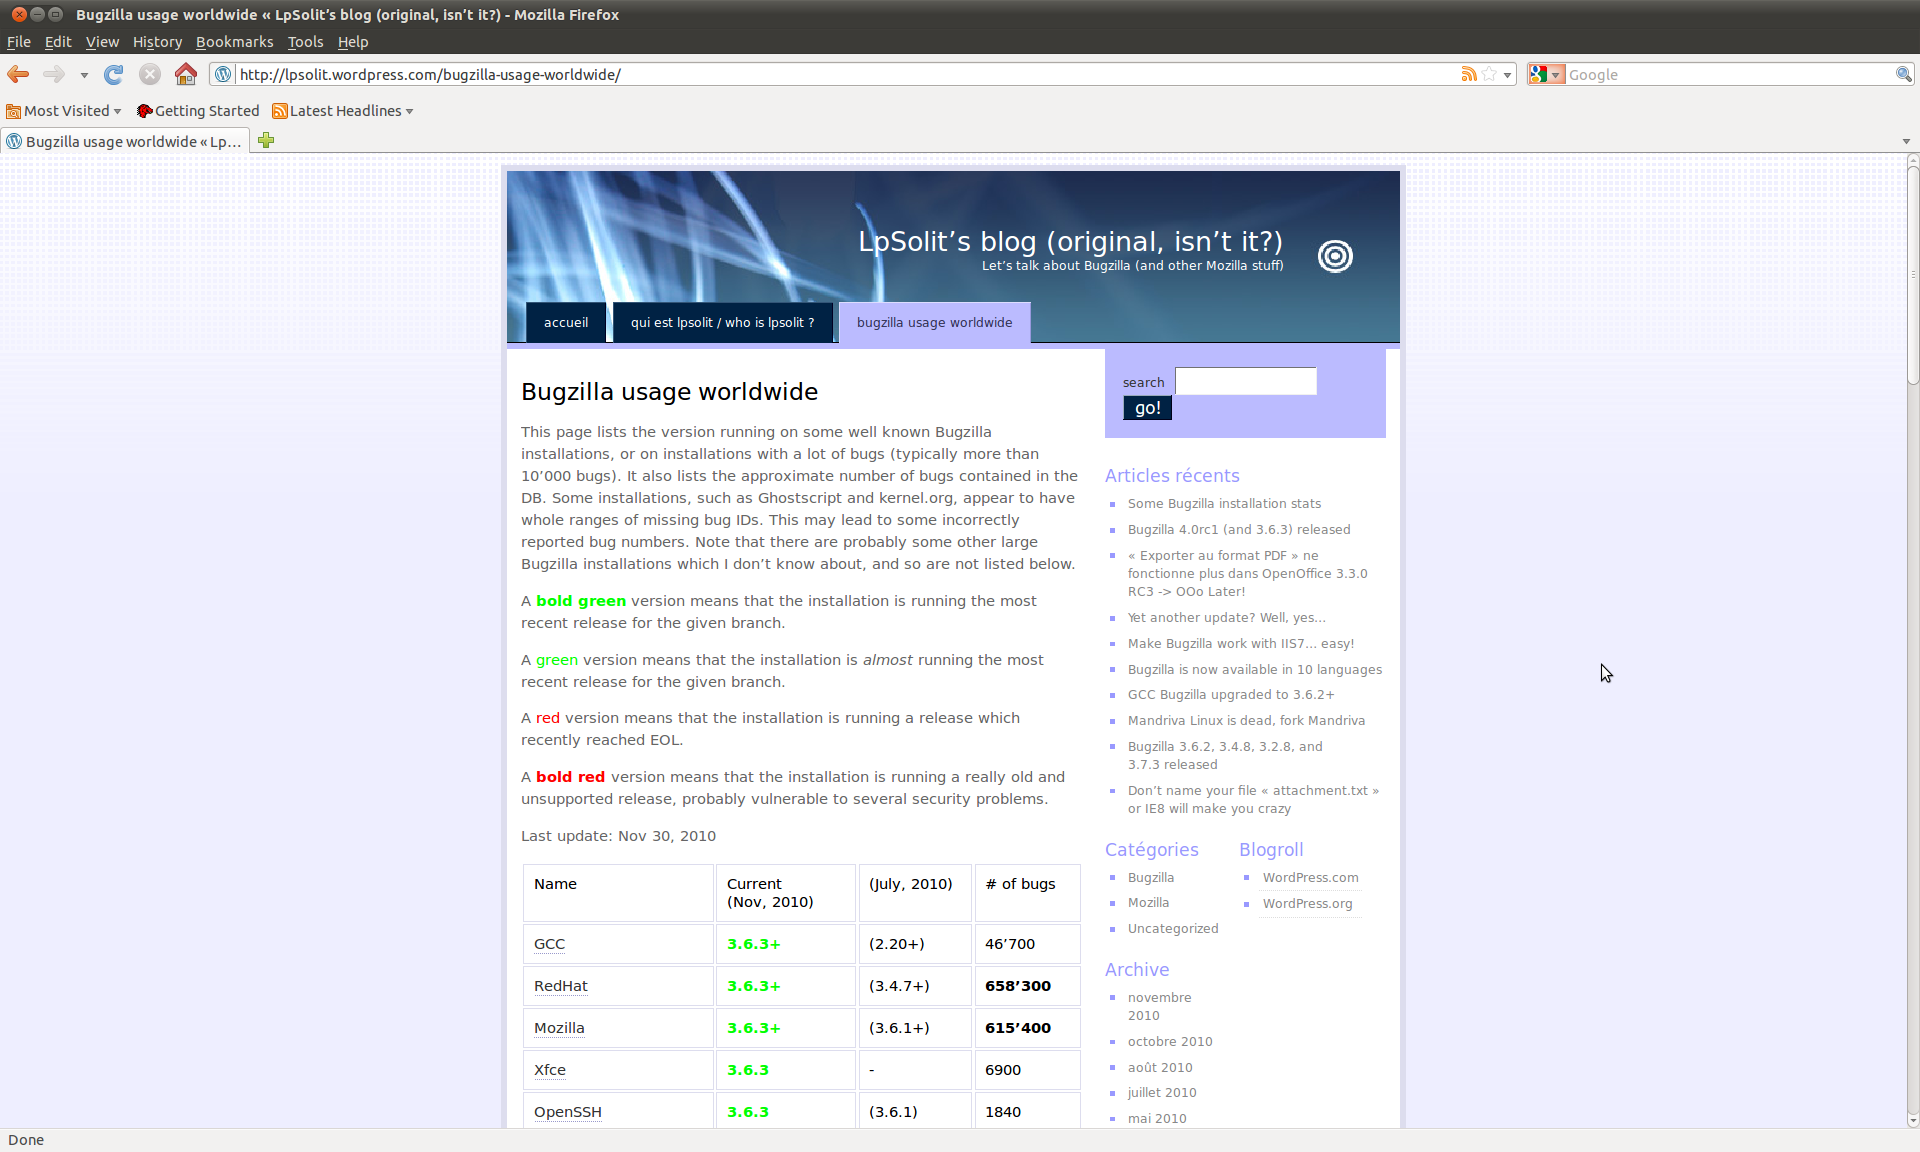
\includegraphics[height=6cm]{figs/Bugzilla_usage_worldwide.png}
\begin{figure}
\end{figure}
\end{center}
\end{frame}

%%%%%%%%%%%%%%%%%%%%%%%%%%%%%%%%%%%%%%%%%%%%%%%%%%%%%%%%%%%%%%

\begin{frame}
\frametitle{Mozilla Install list web page}
\begin{center}
\begin{figure}
 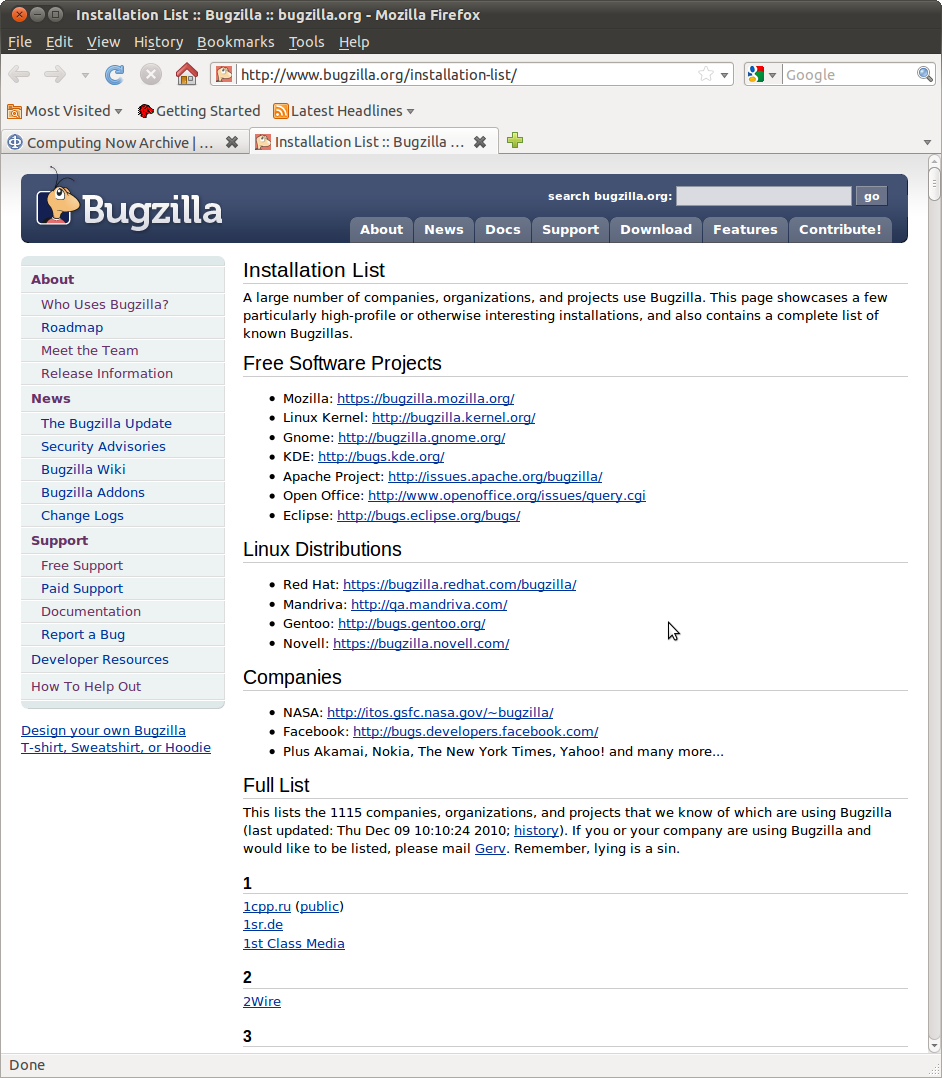
\includegraphics[height=6cm]{figs/Bugzilla_Install_List.png}
\end{figure}
\end{center}
\end{frame}

%%%%%%%%%%%%%%%%%%%%%%%%%%%%%%%%%%%%%%%%%%%%%%%%%%%%%%%%%%%%%%

\begin{frame}
 \frametitle{Mozilla QA Tools: Bugzilla. How to report a bug}
 \begin{itemize}
    \item Point your browser to \textit{http://bugzilla.mozilla.org}
    \item Recomended but not mandatory,have a bugzilla acccount.
    \item Log into bugzilla.
    \item Use the search box in the main page to see if your bug has already been submitted.
    \begin{itemize}
       \item Important to avoid duplicate bugs.
    \end{itemize}
    \item If a previous bug exist, you should add your info into as a comment.
    \item If you are sure that your issue has not already been reported then click in the link New in the toolbar on the top or click the File a bug image.
    \item Select the product in wich you want to fill the bug
 \end{itemize}
\end{frame}

%%%%%%%%%%%%%%%%%%%%%%%%%%%%%%%%%%%%%%%%%%%%%%%%%%%%%%%%%%%%%%

\begin{frame}
 \frametitle{Mozilla QA Tools: Bugzilla. How to report a bug}
 \begin{itemize}
    \item Information needed to report a bug:
    \begin{itemize}
      \item Component. (if you don't know, select 'General').
      \item Version. Of the software that you are using or about you will fill a bug.
      \item Hardware. The architecture of the machine in wich you are running the software.
      \item OS (running the software) Bugzilla will try to guess it!
      \item Summary. A short one-sentence summary of the issue.
      \item Description. Full details of the issue, giving as much detail as possible.
      \item Add and Attachment. Use this button if you have important docs to attach to the bugs, like images or something.
      \item Remember to add all the info that you can, the rest can be left blank).
      \item Once you are done click 'Submmit Bug'.
      \end{itemize}
     \item There is an advance form to report  bug, but it's more complex, using the normal form with the right information should be enought.
     \item Interesting essay about how to fill a bug at \textit{http://www.chiark.greenend.org.uk/~sgtatham/bugs.html}
 \end{itemize}
\end{frame}

%%%%%%%%%%%%%%%%%%%%%%%%%%%%%%%%%%%%%%%%%%%%%%%%%%%%%%%%%%%%%%

\begin{frame}
 \frametitle{Mozilla QA Tools: Crash Reporter}
 \begin{itemize}
 \item Tools that sends information to Thunderbird developers whenever Thunderbird crashes
 \item Is a set of libraries for client-side crash reporting
 \item Same thing, different names
    \begin{itemize}
     \item QFA
     \item TalkBack
     \item BreakPad
     \item Socorro
     \item ...
    \end{itemize}
 \end{itemize}
\end{frame}

%%%%%%%%%%%%%%%%%%%%%%%%%%%%%%%%%%%%%%%%%%%%%%%%%%%%%%%%%%%%%%
\begin{frame}
 \frametitle{Crash Reporter Implementation}
 \begin{itemize}
   \item Client integration to handle crash reporting 
   \item Server (Socorro) that collects and processes collected crash data
   \item A web interface (Socorro) for viewing and parsing crash reports, called
   \item This info is used by Thunderbird developers to make future versions crash less frequently. 
   \item Important part of the Mozilla Core
   \item It cannot be deselected during custom install, unlike the old version, the Talkback add-on.
   \item Also used in other Mozilla products (Firefox, etc).
   \item Development started by Google.
 \end{itemize}
\end{frame}

%%%%%%%%%%%%%%%%%%%%%%%%%%%%%%%%%%%%%%%%%%%%%%%%%%%%%%%%%%%%%%

\begin{frame}
 \frametitle{How to use the crash reporter}
 \begin{itemize}
  \item The Crash Reporter appears only when Thunderbird crashes.
  \item Only when Thunderbird crashes, it doesn't cause Thunderbird to crash!, like some people think.
  \item Once it has appeared, it saves a binary "dump" file, with a lot of info about the crash.
  \item Fill the info in the form to tell Mozilla about this crash so they can fix it.
  \item Mozilla Crash Reporter will send a summary of the crash to Mozilla.
  \item Restart your application!
  \item Referencing crash reports in bugzilla is a good idea, just add the GGUID to the bug, when reporting a bug that cause a crash!
 \end{itemize}
\end{frame}

%%%%%%%%%%%%%%%%%%%%%%%%%%%%%%%%%%%%%%%%%%%%%%%%%%%%%%%%%%%%%%

\begin{frame}
\frametitle{Crash reports: Web view}
 \begin{itemize}
  \item Using Web Interface
     \begin{itemize}
       \item Crash Reporter will save info about all the crashes that happend in your software.
       \item In case of Thunderbird we need a extra extension, view:about is tha man!
       \item about:crashes will show a list with links to all the crashes that your applications has suffered.
       \item Click in one of the links to view the report.
     \end{itemize}
 \end{itemize}
\end{frame}

%%%%%%%%%%%%%%%%%%%%%%%%%%%%%%%%%%%%%%%%%%%%%%%%%%%%%%%%%%%%%%

\begin{frame}
\frametitle{Crash reports: File view}
 \begin{itemize}
  \item Saved a local copy on your system
  \item Locations
    \begin{itemize}
      \item Windows 7/Vista
      \item Windows XP/2000
      \item Mac OS
      \item Linux
    \end{itemize}
  \item Each submitted crash report is identified as a text file, located in the "Crash Reports" folder within the "submitted" subfolder.
  \item Find the GGUID of the crash report that we want to take a look at...
  \item ...append the GGUID to the end of \textit{http://crash-stats.mozilla.com/report/index/}
 \end{itemize}
\end{frame}

%%%%%%%%%%%%%%%%%%%%%%%%%%%%%%%%%%%%%%%%%%%%%%%%%%%%%%%%%%%%%%

\begin{frame}
\frametitle{Mozmill}
 \begin{itemize}
  \item Script testing
  \item Live samples / Videos
 \end{itemize}
\end{frame}

%%%%%%%%%%%%%%%%%%%%%%%%%%%%%%%%%%%%%%%%%%%%%%%%%%%%%%%%%%%%%%


\begin{frame}
\frametitle{Litmus}
 \begin{itemize}
    \item Litmus is a web-based, open source QA tool maintained by Mozilla Corporation.
    \item Is designed to improve workflow, visibility, and turnaround time in the Mozilla QA process.
    \item Everything is manual.
 \end{itemize}

\end{frame}

%%%%%%%%%%%%%%%%%%%%%%%%%%%%%%%%%%%%%%%%%%%%%%%%%%%%%%%%%%%%%%
\begin{frame}
\frametitle{Litmus}
 \begin{itemize}
    \item Litmus does:
       \begin{itemize}
       \item Makes easier for casual testers to assist with testing Mozilla products.
       \item Serve as a repository for test cases, with all the inherent management abilities that implies.
       \item Serve as a repository for test results, carrying over the best features of Testrunner, e.g. test lists, division of labor, etc.
       \item Provide a query interface for viewing, reporting on, and comparing test results.
       \item Expose a web services interface for the mechanical batch submission of testing results.
       \end{itemize}
 \end{itemize}
\end{frame}

%%%%%%%%%%%%%%%%%%%%%%%%%%%%%%%%%%%%%%%%%%%%%%%%%%%%%%%%%%%%%%

\begin{frame}
\frametitle{Litmus}
 \begin{itemize}
    \item Litmus does not:
       \begin{itemize}
       \item Manage the automation of testing.
       \end{itemize}
 \end{itemize}

\end{frame}


%%%%%%%%%%%%%%%%%%%%%%%%%%%%%%%%%%%%%%%%%%%%%%%%%%%%%%%%%%%%%%

\begin{frame}
\frametitle{Title here}
 \begin{itemize}
   \item Example item
 \end{itemize}
\end{frame}

%%%%%%%%%%%%%%%%%%%%%%%%%%%%%%%%%%%%%%%%%%%%%%%%%%%%%%%%%%%%%%

\begin{frame}
\frametitle{Test types}
  \begin{itemize}

  \item Smoketest 
       \begin{itemize}
       \item Covers common operations (Install, Uninstall, Usability)
       \item Includes a set of various operations
       \item Its the Standard Test.
       \end{itemize}
  \item Full Functional Tests
       \begin{itemize}
       \item Its the biggest testrun in Litmus. 
       \item It includes a lot of testcases for all aspects of the Product you have selected.
       \end{itemize}
  \item Localization (l10)
       \begin{itemize}
       \item A test provided for Localization Builds
       \end{itemize}
  \item Basic Functional Test (BFT)
       \begin{itemize}
       \item Includes more testcases than a Smoketest and covers all aspects of the Product.
       \item From Installing till Security Features.
       \end{itemize}

  \end{itemize}
\end{frame}

%%%%%%%%%%%%%%%%%%%%%%%%%%%%%%%%%%%%%%%%%%%%%%%%%%%%%%%%%%%%%%

\begin{frame}
\frametitle{Test results}
 \begin{itemize}
   \item Not Run: The test has not been excuted yet
   \item Pass: Test got the expected results
   \item Fail: Test failed
   \item Test unclear/broken: Not enought information to run the test
 \end{itemize}
\end{frame}

%%%%%%%%%%%%%%%%%%%%%%%%%%%%%%%%%%%%%%%%%%%%%%%%%%%%%%%%%%%%%%

\begin{frame}
\frametitle{Testing...}
 \begin{itemize}
   \item We need a user account in Litmus
   \item A testing build of Thunderfird
   \item Set up for the test run
   \item Execute the test
   \item Submit the test run results
 \end{itemize}
\end{frame}

%%%%%%%%%%%%%%%%%%%%%%%%%%%%%%%%%%%%%%%%%%%%%%%%%%%%%%%%%%%%%%


%%%%%%%%%%%%%%%%%%%%%%%%%%%%%%%%%%%%%%%%%%%%%%%%%%%%%%%%%%%%%%
%%% http://piratepad.net/zyyP4uNTsp
%%%%%%%%%%%%%%%%%%%%%%%%%%%%%%%%%%%%%%%%%%%%%%%%%%%%%%%%%%%%%%

\section{References and Links}

\begin{frame}
 \frametitle{References}
 \begin{itemize}
    \item SuMoMo \textit{http://support.mozillamessaging.com}
    \item SuMo \textit{http://support.mozilla.com}
    \item bugzilla \textit{http://bugzilla.libresoft.es}
    \item breakpad \textit{http://code.google.com/p/google-breakpad/}
    \item crash-stats \textit{http://crash-stats.mozilla.com/report/index/}
    \item Wiki Mozilla \textit{http://wiki.mozilla.org}
  \end{itemize}

\end{frame}

%%%%%%%%%%%%%%%%%%%%%%%%%%%%%%%%%%%%%%%%%%%%%%%%%%%%%%%%%%%%%%

\end{document}
